% !TeX root = ../notes.tex

\section{Textbook Query Optimization}
Textbook query optimization involves techniques to perform a rough first optimization, which however is quite simple. There is a series of steps to translate raw SQL into logical and physical plans, each of them transforming input in a more optimal form.

The output is going to be \textit{executable}, but still to be improved by non-trivial methods.

\subsection{Algebra and tuples}
Plain relational algebra is not sufficient itself: it needs to be revisited ensuring \textbf{correctness} (producing the same result) within a formal model. The most relevant problem to tackle is \textbf{deciding whether two algebraic expressions are the same}, but this in difficult in practice.

For instance, performing a selection before a join might be correct (and faster) in case the considered criterion is equality, but can give a different result than selecting after an outer join. 

To remedy this issue, it is possible to guarantee that two expressions are equivalent, not accepting false positing yet allowing false negatives. 

A formal definition of \textbf{tuple} is an unordered mapping from attribute names to values of a domain. A schema consists in a set of attributes with domain $A(t)$.

Tuple operations are:
\begin{itemize}
	\item \textbf{Concatenation}, attaching one tuple to another regardless of ordering (union);
	\item \textbf{Projection}, producing a notation $t.a$ in which it is possible to access single values or multiple $t_{|\{a, b\}}$, getting a subset of the schema.
\end{itemize}

A set of tuples with the same schema forms a \textbf{relation}. Sets naturally do not comply with real data, since they not allow duplicates, but are used for simplicity.

In most cases, sets and bags can be used interchangeably, but the optimizer considers different semantics: logical algebra operates on \textit{bags}, physical algebra on \textit{streams} and sets are only considered after an \textit{explicit duplicate elimination}.

\begin{figure}
	\begin{minipage}{0.45\textwidth}
		\hspace{-2mm}
		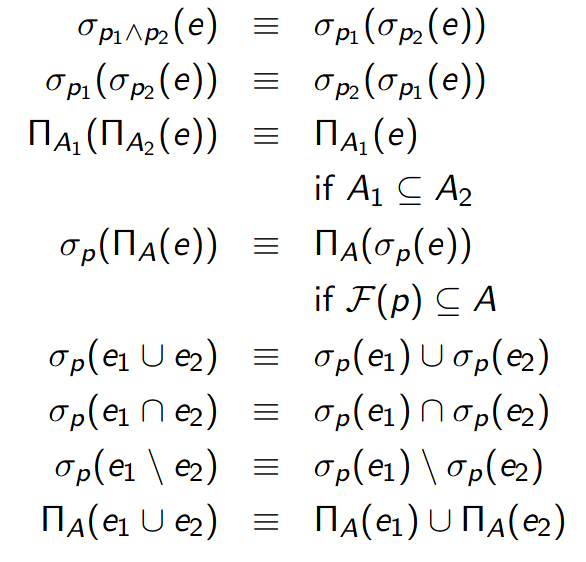
\includegraphics[width=0.83\textwidth]{equivalences_1.png}
	\end{minipage}
	\begin{minipage}{0.5\textwidth}
		\hspace{-10mm}
		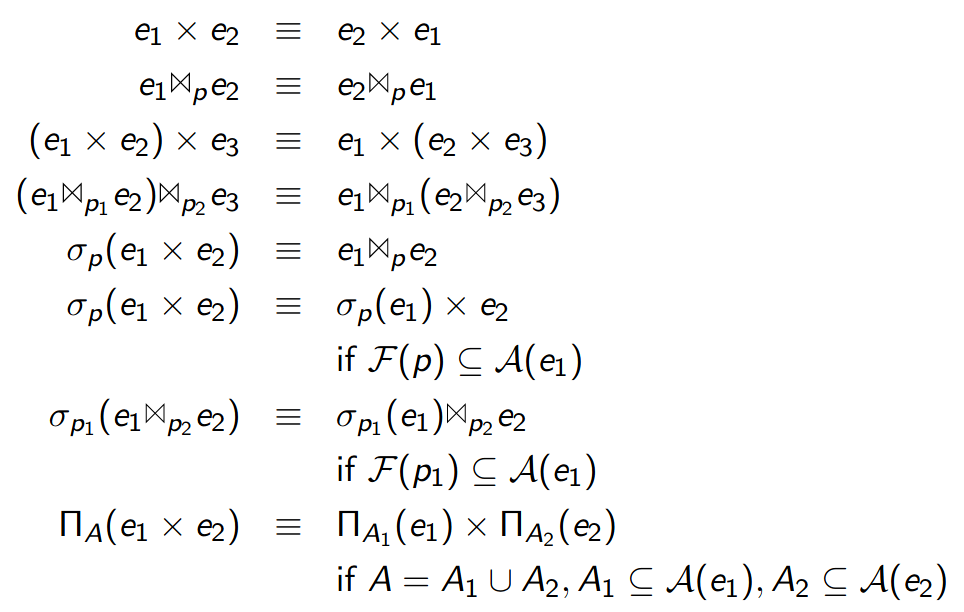
\includegraphics[width=1.2\textwidth]{equivalences_2.png}
	\end{minipage}
	\vspace{-15pt}
\end{figure}

Set operations are the classic ones of union, intersection and difference, yet are \textbf{subject to schema constraints}. On bags, operations are performed on frequencies. 

There are also free variables, which first must be bounded to be evaluated: they are essentials for predicates and algebra expressions, such as dependent joins. 

It is important to note that projection removes duplicates within sets, while keeping them in bags.

There are equivalences for selection and projection useful to derive whether a different ordering produces the same output. For instance, applying selection twice is the same as applying it once with two criteria plus an AND. Commutative property also holds.

\subsection{Canonical Query Translation}
The canonical query translation transforms SQL into \textbf{algebra expressions}. The first approach involves some restrictions: it assumes no duplicates without aggregation and set operations.

The first step is translating the FROM clause:
$$F = \begin{cases}
R_1 & k = 1 \\
((\dots (R_1 \times R_2) \times \dots) \times R_k)) & \text{else}
\end{cases}$$
In short all relations are joined through a cross product. The next step is translating the WHERE clause:
$$W = \begin{cases}
F & \text{there is no WHERE clause} \\
\sigma_p(F) & \text{otherwise}
\end{cases}$$
The SELECT clause is translated starting from the projection $a_1,\ \dots,\ a_n$ or $*$. The expression is constructed:
$$S = \begin{cases}
W & \text{if the projection is ALL} \\
\prod_{a_1,\ \dots,\ a_n}(W) & \text{otherwise}
\end{cases}$$
GROUP BY can also be translated, even though it is not part of the canonical translation. Let $g_1,\ \dots,\ g_n$ be the attributes in the clause and $agg$ the aggregations within SELECT:
$$G = \begin{cases}
W & \text{there is no GROUP BY clause} \\
\Gamma_{g_1,\ \dots,\ g_m:agg}(W) & \text{otherwise}
\end{cases}$$
HAVING is basically the same as WHERE, with the filter predicate on top of $G$.

\subsection{Logical Query Optimization}
Once obtained the relational algebra, equivalences span the \textit{potential search space} and new expressions are derived thanks to them. Of course equivalence can be applied both ways, hence it is relevant to decide which one works better, and conditions have to be checked as well. This, however, makes the search more expensive since there are plenty of alternatives.

To speed the process up, sometimes some equivalences are ignored, even the simplest ones (for instance when choosing the join algorithm).

Query plans can only be compared if there is a cost function, often needing details which are not available merely through relational algebra (what kind of join is being used): logical query optimization is still a \textbf{heuristic} and requires additional steps, since it is not enough to determine the runtime.

Most algorithms, therefore, use the following strategy:
\begin{itemize}
	\item Organization of equivalences into \textbf{groups};
	\item \textbf{Directing equivalences}, deciding the preferred side and rewriting rules to apply them sequentially to the initial expression, trying to reduce the size of intermediate results.
\end{itemize}
For example, a projection on the output of a join can be preferred to a join of a projection. It is important to keep in mind that tuples are being removed in the process, and this only applies in certain circumstances (regular expressions, high selectivity of join).

The rule of thumb is simply to eliminate the most tuples during the intermediate step, to then perform computationally expensive operation with the smallest amount of data.

To summarize, the phases are:
\begin{itemize}
	\item Breaking up conjunctive selection predicates, since simpler predicates can be moved around easier;
	\item Pushing selections down, reducing the number of tuples early;
	\item Introducing joins, which are cheaper than cross product (linear time);
	\item Determining join order, a usually NP-hard problem which is tackled with different approaches;
	\item Introducing and pushing down projections, removing redundant attributes.
\end{itemize}
Some SQL queries have limitations: selections sometimes cannot be pushed down, since there might be no join predicate between tables (cross product). Choosing a different join order allows further push down. 

\subsection{Physical Query Optimization}
Physical query optimization adds execution information to the plan, allowing actual cost calculation and optimizing over data structures, access path and operator implementation.

Data may be sorted or materialized, introducing results which can be reused and deciding where to store them.

First of all, the access path is selected: lookup can be done through \textbf{index} or \textbf{table scan}, depending on the selectivity (fraction of the data satisfying the clause): in general, above 10\% a table scan is recommended. 

Scanning a table might be efficient since tuples are stored adjacent in memory; using index, instead, involves traversing a tree multiple times starting from the root. 

Sometimes it is useful to just store in cache the output of a view, but that also depends on the query plan: intermediate results should actually be reused.

\textbf{Operator selection} is replacing a logical operator with a physical one, according to semantic restrictions (most operators require equi-join).

A blockwise nested loop join is generally better than a natural join; sort merge join and hash join are better than both. In general, hash join is the best if not reusing sorts. This process must be performed for all operators: sort join requires ordered tuples, distributed databases need local data and there are multiple ways to model the properties (hashing).

Sort merge join might outperform the hash join if the amount of data is much larger than the available memory.

Materializing, on the other side, is quite relevant for nested loop joins: the first pass is expensive, but the afterwards ones are way cheaper, making it essential for multiple consumers. 
